%
\documentclass[conference]{IEEEtran}
\usepackage{times}

% numbers option provides compact numerical references in the text. 
\usepackage[numbers]{natbib}
\usepackage{multicol}
\usepackage[bookmarks=true]{hyperref}
\usepackage{color}
\usepackage{graphicx}
%\usepackage{subfloat}
\usepackage{textcomp}
\usepackage{amsthm}
\usepackage{amsfonts}
\usepackage{subcaption}
\usepackage{algorithm}
\usepackage{algpseudocode}
\usepackage{pbox}
\usepackage[normalem]{ulem}

\theoremstyle{definition}
\newtheorem{definition}{Definition}[section]
\usepackage{amsmath}

\renewcommand{\algorithmicrequire}{\textbf{Input:}}
\renewcommand{\algorithmicensure}{\textbf{Output:}}

%% Tarik's Shortcuts
% For marking TODOs in an obvious way
\newcommand{\TODO}[1]{ {\bf \textcolor{red}{TODO:} #1 }}
\newcommand{\abj}[1]{\textcolor{blue}{#1}}
\newcommand{\dbj}[1]{\textcolor{blue}{\sout{#1}}}
\newcommand{\cbj}[2]{\textcolor{blue}{\sout{#1}}\textcolor{blue}{~#2}}
\newcommand{\abt}[1]{\textcolor{magenta}{#1}}
\usepackage{amsbsy}

\begin{document}

% paper title
\title{Computer-aided Compositional Design and Verification for Modular Robots}

% You will get a Paper-ID when submitting a pdf file to the conference system
\author{Author Names Omitted for Anonymous Review. Paper-ID [add your ID here]}

\maketitle

\begin{abstract}
In this paper, we present a software framework for the compositional design of
modular robot configurations and behaviors. Designs are constructed
hierarchically by composing elements from a library, allowing users to easily
create complex designs.  Likewise, complex behaviors are constructed by
composing controllers from a library in a nested series/parallel structure. The
system is integrated with a full dynamic simulator, and provides tools to automatically
identify common problems with behaviors, specifically self-collision and loss
of gravitational stability.

\end{abstract}

\section{Introduction}
Modular reconfigurable robot systems have been studied extensively for several
decades \TODO{citations}.  These systems distinguish themselves from conventional robotic systems in their
ability to transform into different shapes to address a wide variety of tasks. \abt{They
promise to be versatile, robust, and low cost \cite{yim2000polybot}. Dozens of groups
have different kinds of reconfigurable robots \cite{fukuda1990cellular, lipson2000towards}, and introduced approaches
for programming them \cite{salemi2001hormone, walter2002choosing, melek2003neurofuzzy}.  Over 800 papers, a book \cite{stoy2010book}, and a survey \cite{yim2007modular}
have been written on the subject. }

This versatility places an additional burden on the user, because
solving problems with modular robots involves not only designing  programs,
but also the best physical form for the task at hand. If this
complexity is not appropriately managed, it will present a significant barrier to
using modular robots to address practical tasks \cite{yim2000modular}. If the user is free to create any new design to
solve a new task, but must program the design from scratch every time, creating
new designs will be a huge amount of effort, and the advantage of versatile modular
hardware will be defeated. \TODO{Add examples from challenges}

Software modularity is a well-established practice for developing large
maintainable systems and avoiding duplication of effort \TODO{cite}. In robotics, software
behaviors are inextricably linked to the hardware they control, resulting in
additional challenges to making modularity effective. Significant progress has been made in
sharing robotics software between researchers
and hardware platforms, most notably
ROS \cite{Quigley2009} which provides inter-process communication and standard libraries for common robot tasks. 

The challenges of designing behaviors are different in modular robotics than
in typical robotics, because the hardware itself is modular. Porting software
from one robot platform to a completely different robot platform takes a
considerable amount of time, and needs to be facilitated by a large framework
such as ROS, in which fundamental software libraries are almost totally decoupled from
specific hardware. In modular robotics, the emphasis needs to be on speed of
design, because the major advantage of a modular robot system is that new
designs can be made for each task. We need to  very quickly develop simple kinematic
behaviors (\textit{e.g.} take a step with a leg) with new morphologies that share some of the
structure of old morphologies.

Our solution to this problem is to let the modularity of our hardware guide the
modularity of our behaviors. We create new modular robot designs by combining existing sub-designs,
for example combining four legs with a body to create a walking robot.
We provide a GUI tool that allows users to do this easily. Designs have
associated libraries of behaviors, so that when new designs are created
by composing existing sub-designs, new behaviors for that design can be quickly
and easily created by composing the behaviors associate with its component
sub-designs. We introduce a new behavior composition formalism with a series-parallel
execution structure that allows old behaviors to be easily and clearly combined
into new behaviors.

Since combining old things in new ways can lead to unexpected problems, we also
need to verify that our new designs and behaviors perform the way we expect them
to. This is done in a dynamic simulation in Gazebo, and through
verification tools that detect common problems. \TODO{Integrate into intro}


\section{Contribution and Paper Structure}

The primary contribution of this paper is a formalism for the construction of modular
robot configurations and behaviors by composition, and a simulation
environment that helps the user verify intended behavior.  Together, these tools
help manage the complexity of a modular robot system, significantly reducing the
time and effort required to develop sophisticated configurations and behaviors.  The software we
have developed is open-source and will be made freely available online.

The remainder of this paper provides a  description of the
structure and algorithmic components of our design framework.  In Section \ref{sec:related-work},
we discuss relevant background material.
In Section \ref{sec:preliminaries} we introduce terminology and  concepts used elsewhere in the
paper. 
In Section \ref{sec:approach}, we describe the algorithmic basis
for the three major components of our framework - design composition, behavior
composition, and behavior verification.  In Section
\ref{sec:example}, we discuss the open-source software
tools used to implement our framework, and provide examples demonstrating a user's
workflow when using this system.  We demonstrate that our framework saves the
user time and effort, and allows him or her to easily develop complex and
capable designs.


\section{Related Work}
\label{sec:related-work}
In some respect\abj{s}, our work parallels the efforts of Mehta \cite{mehta2014design}
and Bezzo \cite{bezzo2014demo}, who aim to create and program printable robots from
novice users' design specifications.  Users create new designs by composing
existing elements from a design library, and appropriate circuitry and
control software are automatically generated as physical designs are assembled. The framework we present is
intended specifically for modular robots, and consequently the workflow and design considerations are fundamentally different
from that presented by Mehta and Bezzo.  In
traditional robot design (or printable robot design), hardware and software are somewhat
decoupled - hardware is
designed and built once, and then programmed many times.  In the case of a modular robot system, the system can be reconfigured to meet new tasks,
so hardware configuration and behavior programming go hand in hand.  We intend
our system to be fast enough that the user could conceivably develop and program
a new design for every new task - designs are built once, and programmed once.  Where Mehta et al. provide many facilities to generate and verify
low-level behaviors (\textit{e.g.} motor drivers appropriate for motors), we do so for
high-level behaviors.

A significant amount of work has been done in developing behaviors and software
for modular robots. Much of this work focused on automatically
generating designs and behaviors using artificial intelligence systems. Genetic
algorithms have been applied for the automated generation of designs
and behaviors \cite{hornby2003generative}. Other work has
focused on emergent behavior from distributed algorithms \TODO{cite papers}.

While significant progress has been made in the automated generation of modular robot behaviors,
automated systems are not yet capable of making modular robots truly useful in practice
\cite{yim2007modular}.  The need for new programming techniques to manage the complexity
of modular robot systems has been acknowledged in the literature \cite{yim2000modular}.
Historically, gait tables have been a commonly used format in which open-loop kinematic
behaviors can be easily encoded \cite{yim1994locomotion}. Phased automata have also
been presented as a way to easily create scalable gaits for large numbers of modular
robots \cite{zhang2003phase}. \abt{In this paper, we introduce a novel motion description
language that enables users to quickly create behaviors for modular robots}.

Our framework assists users in verifying design validity by identifying self-collision
and loss of gravitational stability. \abt{In existing literature, these conditions have
been checked in the context of modular robot reconfiguration planning \cite{casal2001reconfiguration} and motion
planning \cite{yoshida2002self}.
To our knowledge, there is no modular robot design tool that verifies
these conditions to provide assistance to a human designer.}

\section{Definitions}
\label{sec:preliminaries}
In this section, we present concepts and terms which will be used later in the paper.

\begin{definition}[Module] A module is a small robot that can move, respond to commands,
and attach to other modules.  Formally, we define a  module  as $\mathcal{M}=({^\mathcal{W}}D^{\mathcal{M}}, X, A,
K)$, where:
\begin{itemize}
\item ${^\mathcal{W}}D^{\mathcal{M}}\in SE(3)$ is the rigid-body \textit{displacement} (position and orientation)
of the module body frame in the world reference frame $\mathcal{W}$. 
\item \(X=\lbrace x_1, x_2, \ldots, x_d \rbrace\) is the \textit{state} of the module,
with each \(x_i\) corresponding to one of the \(d\) degrees of freedom (DoF) of the module.
\item $A=\{a_1, a_2, ..., a_k\}$ is the set of \textit{attachment points} where the module can connect to other modules.
\item \(K: (X, a_i) \rightarrow SE(3) \) is the module's \textit{forward kinematics function}, returning \({^\mathcal{B}}D^{a_{i}}\) (the displacement of attachment point \(a_i\)
in the body frame) as a function of \(X\)  \end{itemize}

Figure~\ref{fig:smores} shows a schematic representation of a module with  four attachment points
\end{definition}

\begin{figure}
\begin{center}
        \begin{subfigure}[b]{0.4\columnwidth}
                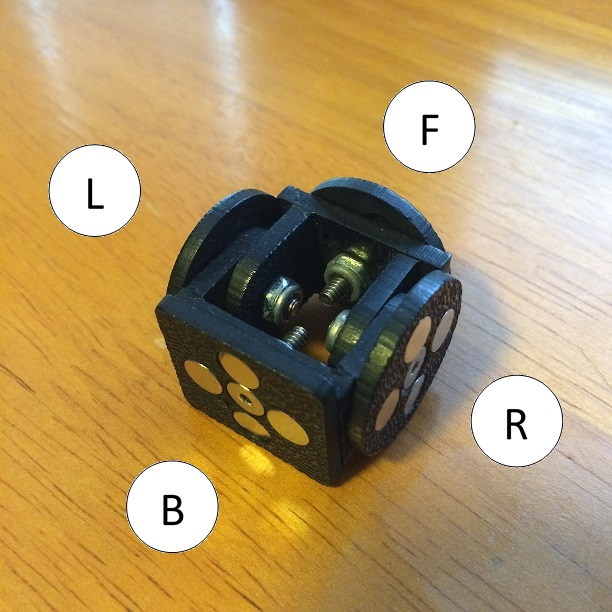
\includegraphics[width=\textwidth]{images/smores.JPG}
                \caption{A module}
                \label{fig:smores_photo}
           \end{subfigure}
           ~
        \begin{subfigure}[b]{0.4\columnwidth}
                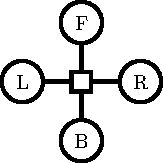
\includegraphics[width=\textwidth]{images/tikz/smores.pdf}
                \caption{The graphical representation}
                \label{fig:smores_graph}
        \end{subfigure}
\end{center}
\caption{A photo of a module and its graphical representation}
\label{fig:smores}
\end{figure}


\begin{definition}[Configuration]
\label{def:configuration}
A \textit{configuration} is a contiguous set of connected modules which we treat as a
single robot.  The identity of a configuration is determined by its connective structure; configurations
can be represented by graphs with nodes representing modules and edges
representing connections between modules.   Individual modules
are considered interchangeable (as long as they are of the same kind).

In this paper, we present an object-oriented design framework for modular robot
systems, and treat configurations as the fundamental objects. Rather than defining
configurations only by the topology of their component modules, we define them recursively,
as being composed of connected sub-configurations. A single module is considered the
smallest configuration.

Formally, we define a configuration as $\mathcal{C}=(C_, \gamma, M, E, \delta,
X, B)$, where:
\begin{itemize}
\item $C$ is a set of sub-configurations, $C=\{\mathcal{C}_{1}, \mathcal{C}_{2}, ..., \mathcal{C}_{q}\}$.
\item $\gamma: C \rightarrow M$ is a function {mapping} a configuration \( \mathcal{C}
\in C\) to its set
of modules.
% Note: if we define a single module as the smallest configuration, we don't have
% to worry about the case when the configuration contains no configurations.
\item \( M=\bigcup_{\mathcal{C}\in C}{\gamma(\mathcal{C})} \) is the set of modules.
%\item $M$ is the set of modules. If this configuration contains no other configurations, i.e. $C = \emptyset$, $M$ is just the set of all modules of this configuration. If this configuration is composed by other configurations, i.e. $C=\{\mathcal{C}_{1}, \mathcal{C}_{2}, ..., \mathcal{C}_{q}\}$, we define $M=\bigcup_{\mathcal{C}\in C}{\gamma(\mathcal{C})}$.
\item $E$ is a set of connections between modules. $(\mathcal{M}_i.a_i, \mathcal{M}_j.a_j)\in E,$ where $\mathcal{M}_{i},\mathcal{M}_j \in M, \mathcal{M}_i \neq \mathcal{M}_j$, and $a_i\in \mathcal{M}_i.A$, $a_j\in \mathcal{M}_j.A$.
\item $\delta: E \rightarrow SO(3)$ is a labeling function over connections returning
\({^{\mathcal{M}_i.a_i}}R^{\mathcal{M}_j.a_j}\), the \abt{orientation} of one attachment point relative the
other. \item \(X = \displaystyle\bigcup_{\mathcal{M}_i \in M} \mathcal{M}_i.X \) is the \textit{state} of the configuration.
\item \(B\) is a set of \textit{behaviors} (Definition~\ref{def:behavior}) associated with the configuration.
\end{itemize}

Figure~\ref{fig:smores_conf_photo} shows a photo of a configuration composed
of three modules, each with four attachment points.  Figure~\ref{fig:smores_conf_graph} shows its
graphical representation. Blue zigzag lines represent connections between
modules, and the label of each connection shows the angle offset of that
connection.

In this paper, we consider only configurations without cycles. While this is a constraint,
the \abt{set of functionalities provided by acyclic designs is very rich, so we feel that
it does not unreasonably limit the utility of our framework. Accomodating designs
with cycles is left to future work.}

Assuming acyclic configurations, we can compute forward kinematics for the entire
configuration by composing displacements module-to-module. Let any module \(\mathcal{M}_f \in M\) have
fixed displacement \({^\mathcal{W}}D^{\mathcal{B}_f}\) in the world frame.
Let \(\mathcal{M}_i: (\mathcal{M}_i.a_i,~\mathcal{M}_f.a_f) \in E \) be connected to \(\mathcal{M}_f\).
 We can find \({^\mathcal{W}}D^{\mathcal{M}_i}\) by composing displacements as follows:
\begin{align*}
{^\mathcal{W}}D^{\mathcal{M}_i} =& [{^\mathcal{W}}D^{\mathcal{M}_f}] [{^{\mathcal{M}_f}}D^{a_f}][
{^{a_f}}D^{a_i}] [{^{\mathcal{M}_i}}D^{a_i}]^T \\
=& [{^\mathcal{W}}D^{\mathcal{M}_f}] [K_f(X_f,a_f)] \begin{bmatrix} \delta(e) & 0
\\ 0 & 1\end{bmatrix} [K_i(X_i,a_i)]^T
\end{align*}

where \(e=(\mathcal{M}_i.a_i,~\mathcal{M}_f.a_f)\). To find the world-frame displacements
of all other modules, we may traverse the connections of the configuration,  repeatedly
composing displacements in the manner above.
\end{definition}

\begin{figure}
\begin{center}
        \begin{subfigure}[b]{0.4\columnwidth}
                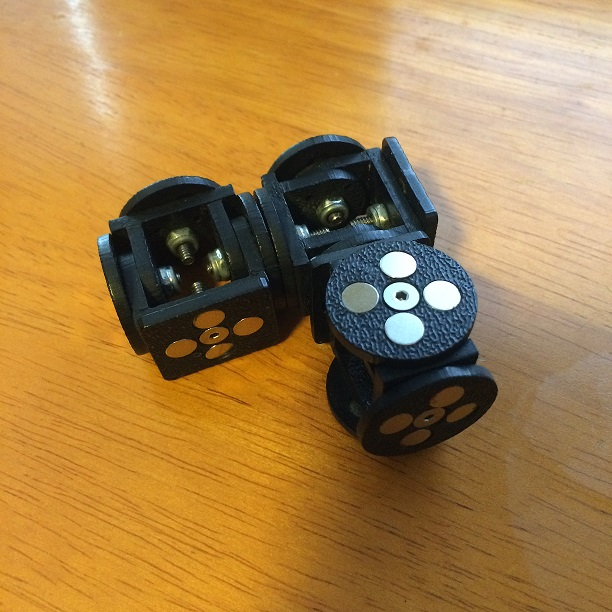
\includegraphics[width=\textwidth]{images/smores_conf.JPG}
                \caption{A configuration}
                \label{fig:smores_conf_photo}
           \end{subfigure}
           ~
        \begin{subfigure}[b]{0.4\columnwidth}
                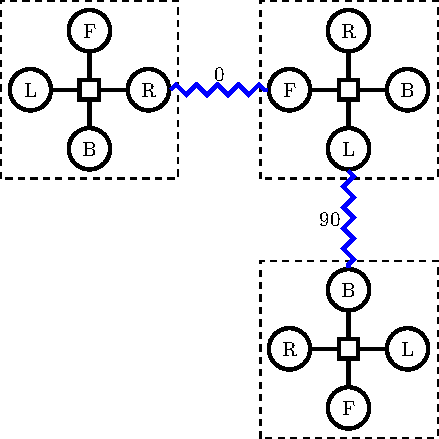
\includegraphics[width=\textwidth]{images/tikz/smores_conf.pdf}
                \caption{The graphical representation}
                \label{fig:smores_conf_graph}
        \end{subfigure}
\end{center}
\caption{A photo of a configuration with three modules and its graphical representation}
\label{fig:smores_conf}
\end{figure}



\begin{definition}[Behavior]\label{def:behavior}
A \textit{behavior} is a programmed sequence of movements for a specific configuration
intended to produce a desired effect.  A gait for walking is one example.  In
this paper, we consider open-loop kinematic behaviors represented as
series-parallel action graphs, described in detail in section
\ref{sec:behavior-representation}.
\end{definition}
\begin{definition}[Controller]
A \textit{controller} is a position or velocity servo for one DoF of a modular
robot.  A controller takes as input a desired position or angular velocity, and
drives the error between the desired and actual state of the DoF it controls to
zero over time.
\end{definition}
\begin{definition}[Behavior Conflict]
When writing a behavior, it is possible to command one controller to
simultaneously hold more than one desired position; this is known as a
\textit{behavior conflict}.  Behaviors with conflicts are
impossible to execute.
\end{definition}
\begin{definition}[Self-Collision]
During execution of a behavior, a \textit{self-collision} can occur when two
different parts of configuration are commanded to occupy the same location in
space.  Self-collisions can damage the robot, and are usually unwanted.
\end{definition}
\begin{definition}[Gravitational Stability]
While executing many behaviors, it is desirable to maintain \textit{gravitational
stability} (also called quasi-static stability).  Informally speaking, a
robot is gravitationally stable when it is balanced, and gravity does not
create any net moment on it.  Mathematically, the robot is gravitationally stable
if the projection of its center of
mass onto the group plane lies within the convex hull of its load-supporting contact points in the
ground plane.
\end{definition}

\section{Approach and Algorithm}
\label{sec:approach}
The three major components of our framework are configuration composition, behavior
composition, and verification of configurations and behaviors. 
\subsection{Configuration Composition} \label{sec:conf_composition}


\begin{definition}[Configuration Composition]
Given a set of configurations $C$ %, a base configuration $\mathcal{C}_b\in C$, 
and a set \ $E_C$ of connections between them, configuration composition
combines all configurations in $C$ to a single configuration $\mathcal{C}^*$
that
%has the following guarantees: i) $\mathcal{C}^*$ 
includes all modules and
connections from $C$ and $E_C$.% (section~\ref{sec:update_connection})
% ; ii) the
% positions of all modules in $\mathcal{C}^*$ are adjusted based on the
% connections to preserve structures of original configurations in $C$
% (section~\ref{sec:update_position}).
\end{definition}
%\subsubsection{Update Modules and Connections} \label{sec:update_connection}
%Before presenting the procedure to update modules and configurations in $\mathcal{C}^*$, we will first discuss some assumptions about the set of connections $E_C$.
The set of connections $E_C$ between configurations in $C$ is defined as $(\mathcal{C}_i.\mathcal{M}_i.a_i, \mathcal{C}_j.\mathcal{M}_j.a_j) \in E_C$, where $\mathcal{C}_{i,j}\in C$, $\mathcal{M}_i \in \gamma(\mathcal{C}_i), \mathcal{M}_j \in \gamma(\mathcal{C}_j)$, and $a_i\in \mathcal{M}_i.a$, $a_j\in \mathcal{M}_j.A$. Similar to the assumption about connections in a configuration, we assume that if we form an
acyclic graph with configurations in $C$ as nodes and connections in $E_C$ as edges.

Given a set of configurations $C$ %, a base configuration $\mathcal{C}_b\in C$, 
and a set of connections $E_C$, we define the composed configuration to be $\mathcal{C}^*=(C^*, \gamma, M, E, \delta,
X, B)$, where
\begin{itemize}
\item $C^*=C$
\item $M=\bigcup_{\mathcal{C}\in C^*}{\gamma(\mathcal{C})}$.
%\item $\mathcal{M}_b\in M$ is the base module of the base configuration $\mathcal{C}_b$.
\item $E= (\bigcup_{(\mathcal{C}_i.\mathcal{M}_i.n_i, \mathcal{C}_j.\mathcal{M}_j.n_j)\in E_C}{\{(\mathcal{M}_i.n_i, \mathcal{M}_j.n_j)}\})$ $\cup$ $(\bigcup_{\mathcal{C}_i \in C^*}{E_{i}})$
\item \(B = \bigcup_{\mathcal{C}_i \in C} B_i\)
\end{itemize}
The definitions of $\gamma$, \(X\), and $\delta$ are the same as the ones in Definition~\ref{def:configuration}.
% \subsubsection{Update Positions of all Modules} \label{sec:update_position}
% As multiple configurations are combined, positions and orientations of some modules in them need to be changed to preserve the relative positioning between modules as in the original configurations.
% 
% \begin{algorithm}
% \caption{Update Module Position}\label{alg:update_position}
% \begin{algorithmic}[1]
% \Require
% \Statex A parent module $\mathcal{M}_p$
% \Statex A child module $\mathcal{M}_c$
% \Statex A connection $e=(\mathcal{M}_p.n_p, \mathcal{M}_c.n_c)$ and the labeling function $\delta$
% \Ensure
% \Statex The child module $\mathcal{M}_c$ with position and orientation updated
% \Statex
% \State c\_wrt\_p $\gets$ get\_transform($\mathcal{M}_p.V_p$, $\mathcal{M}_p.V_p$, $e$, $\delta$) \label{line:1}
% \State p\_wrt\_world $\gets$ get\_matrix($\mathcal{M}_p.P_p$, $\mathcal{M}_p.O_p$) \label{line:2}
% \State c\_wrt\_world $\gets$ p\_wrt\_world $\cdot$ c\_wrt\_p \label{line:3}
% \State $\mathcal{M}_c.P_c \gets$ get\_position(c\_wrt\_world) \label{line:4}
% \State $\mathcal{M}_c.O_c \gets$ get\_orientation(c\_wrt\_world) \label{line:5}
% \State \Return $\mathcal{M}_c$
% \end{algorithmic}
% \end{algorithm}
% 
% \begin{algorithm}
% \caption{Update All Module Positions}\label{alg:update_all_positions}
% \begin{algorithmic}[1]
% \Require
% \Statex A configuration $\mathcal{C}$
% \Ensure
% \Statex The configuration $\mathcal{C}$ whose module positions are all updated
% \Statex
% \State $\mathcal{M}_p \gets \mathcal{C}.\mathcal{M}_b$ \label{line:6}
% \State $M=\{\mathcal{M}_p\}$ \label{line:7}
% \State $\mathcal{C}.M=\emptyset$ \label{line:8}
% 
% \While{$M\neq\emptyset$} \label{line:9}
% \For{$(\mathcal{M}_i.n_i, \mathcal{M}_j.n_j) \in \mathcal{C}.E$} \label{line:10}
% \If{$\mathcal{M}_i=\mathcal{M}_p$} \label{line:11}
% \State $\mathcal{M}_j=$~UpdateModulePosition$($ \label{line:12}
% \Statex \hspace{3cm}$\mathcal{M}_i, \mathcal{M}_j, (\mathcal{M}_i.n_i, \mathcal{M}_j.n_j), \mathcal{C}.\delta)$
% \State $M=M\cup\{\mathcal{M}_j\}$ \label{line:13}
% \State $\mathcal{C}.M=\mathcal{C}.M\cup\{\mathcal{M}_j\}$ \label{line:14}
% \EndIf \label{line:15}
% \EndFor \label{line:16}
% \State $M=M \setminus \{\mathcal{M}_p\}$ \label{line:17}
% \State $\mathcal{M}_p \gets$ RandomOneFrom$(M)$ \label{line:18}
% \EndWhile \label{line:19}
% 
% \State \Return $\mathcal{M}_c$
% \end{algorithmic}
% \end{algorithm}
% 
% Given a parent module $\mathcal{M}_p$, a child module $\mathcal{M}_c$, the connection between them and the corresponding labeling function, Algorithm~\ref{alg:update_position} updates the position and orientation in the global reference frame of the child module based on the relative positioning between $\mathcal{M}_p$ and $\mathcal{M}_c$. Function ``get\_transform'' in line~\ref{line:1} computes the transformation matrix for the reference frame from the parent module to the child module. Function ``get\_matrix'' in line~\ref{line:2} computes the transformation matrix from global frame to the parent module frame. With the two transformation matrices, line~\ref{line:3} computes the transformation matrix from the global frame to the child module frame. In line~\ref{line:4}, \ref{line:5}, functions ``get\_position'' and ``get\_orientation'' update the position and orientation of the child module.
% 
% With the algorithm to update the position and orientation between two modules, Algorithm~\ref{alg:update_all_positions} shows the procedure to update the position and orientation of all modules in a given configuration $\mathcal{C}$. The algorithm starts with the base module of $\mathcal{C}$ as shown in line~\ref{line:6}. $M$ is the set of modules who are updated already, but some modules that are directly connected to modules in $M$ are not updated yet. The set of modules of $\mathcal{C}$ is reset to the
% empty set in line~\ref{line:8}. The while loop from line~\ref{line:9} to \ref{line:19} ensures all modules in $\mathcal{C}$ are updated. The for loop and if statement in line~\ref{line:10}, \ref{line:11} find all connections in $\mathcal{C}.E$ whose first module is $\mathcal{M}_p$. In line~\ref{line:12} we apply Algorithm~\ref{alg:update_position} to update the position and orientation of the second module in those connections. Line~\ref{line:13}, \ref{line:14} append the updated module into the set $M$ and $\mathcal{C}.M$. In line~\ref{line:17}, \ref{line:18}, we remove the current $\mathcal{M}_p$ from the set $M$ and randomly choose a new $\mathcal{M}_p$ from $M$. Notice that the assumption we made about connections of a configuration in Definition~\ref{def:configuration} prevents us from updating the same module twice.
\subsection{Behavior Composition: Series-Parallel Action Graphs}
\label{sec:behavior-representation}
We present a novel motion description language for modular robots.  The
language aims to balance simplicity and expressiveness, and is compositional in
nature, designed to manage the complexity of developing complicated behaviors
for large clusters of modular robots through abstraction and modularity. 
The language is in some ways similar to typical motion description languages, which have atomic elements that represent controller
commands (set-points and gains) with limited duration \cite{brockett1988computer}.
Extended motion description languages introduce interrupts to control the duration
of commands \cite{hristu2003motion}.  The atomic commands of our language have unlimited
duration (until they are superseded by another command), and each apply to a single
DoF of the robot.
%These properties allow complex behaviors to be created through composition operations.
\TODO{Talk about the reason we are using SPAG's rather than something
else.}

 The fundamental atoms of the language are called actions.  An \textit{action} is a tuple \(
(J, X, \xi, T)\), where \(J\) identifies a single DoF of a configuration, \(X\) is a
controller setpoint for that DoF, \(\xi\) specifies an interrupt
condition, and T specifies a timeout. When an action executes, the controller
setpoint (position or velocity) for the specified DoF is changed to the specified
value. The controller maintains this setpoint until receiving a new one from another
action. The interrupt condition is a boolean function of the (sensed) state of the DoF \(J\).
When either the interrupt condition is met or time runs out (whichever comes
first), the action is considered complete, and the next action  begins. The
interrupt condition can be set to \(false\) (so that only the timeout has effect),
and \(T\) can be set to infinity (so that only the interrupt has effect). As an example,
the action \((~Module0\_L,~ \theta_{set}=\pi,~ \xi:\theta==\pi,~T:\infty~)\) encodes
``Command the controller of the left wheel of module zero to maintain a setpoint
of \(\pi\) radians.  When the encoder of that wheel indicates that \(\pi\) radians \TODO{unfinished}
 
Actions are composed to form behaviors. We define a \textit{behavior} as a directed acyclic graph where nodes are
actions and edges are transitions between actions.  A behavior \(B\) always has
two special nodes \(S\) and \(T\), which are the \textit{Start} and
\textit{Termination} nodes, respectively.  The smallest behavior consists of
\(S\), \(T\), and a single action.  Behavior execution follows three simple
rules:

\begin{enumerate}
\item Execution begins at \(S\).  \(S\) completes immediately.
\item Each action begins execution upon completion of \textit{all} its parent actions.
\item All sequences of execution end at \(T\).
\end{enumerate}

Because execution begins at \(S\) and ends at \(T\), there must be a (directed)
path from every \(S\) to every node in \(B\), and also from every node in \(B\)
to \(T\). Since \(B\) is acyclic, it is therefore a \textit{directed series-parallel graph} (SPG).
SPG's can always be formed recursively by parallel and series composition
operations \cite{valdes1979recognition}. The parallel composition \(P\) of two behaviors \(B_1\),
\(B_2\), \(P = Pc(B_1, B_2)\) is the disjoint union of their nodes (actions),
merging \(S_1\) with \(S_2\) and \(T_1\) with \(T_2\). The series composition
of \(B_1\), \(B_2\), \(S = Sc(B_1, B_2)\) is created from their disjoint union
by merging \(T_1\) and \(S_2\), so that \(B_1\) and \(B_2\) execute
sequentially\footnote{Since the merged node is not an action, we can freely
omit it and instead draw edges from each of its parent nodes to each of its
child nodes.}.  Note that if \(B_1\) was itself created through parallel
composition, \(B_2\) will not begin until all chains of execution of \(B_1\)
are completed. Figure \ref{fig:graph-composition} provides a visual companion.

\begin{figure}
\begin{center}
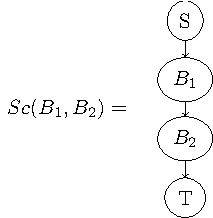
\includegraphics[height=0.8in]{images/tikz/series.pdf}
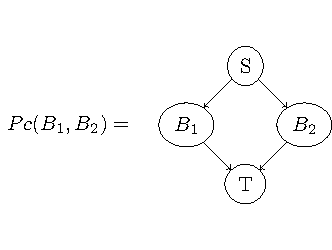
\includegraphics[height=0.8in]{images/tikz/parallel.pdf} \vspace{0.in}
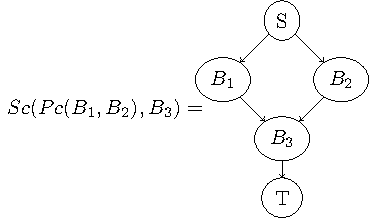
\includegraphics[height=0.8in]{images/tikz/parallel-and-series.pdf}
\end{center}
\caption{Series and parallel composition of behaviors }
\label{fig:graph-composition}
\end{figure}

\subsubsection*{Example}
Consider a single module that has two wheels that allow it to drive like a car. To
drive forward, we might define a DRIVE behavior composing actions for  the left and right wheels
in parallel:\begin{align*}
\mathrm{DRIVE} =~~~~~~~~~~~~~~~~~~~~~~~~~~~~~~~~~~~~~~~~~~~~~~~~~~~ \\
Pc \left( \begin{array}{cccc}
(~L, & \dot\theta_{set}=6, & \xi:false, & T:5), \\
(~R, & \dot\theta_{set}=6, & \xi:false, & T:5) \\
\end{array} \right)\\
\end{align*}
The wheels are set to turn at 6 radians per second, and the action will complete
in 5 seconds.  We might also define a TURN behavior, commanding the wheels to rotate \(\pi\) radians
in opposite directions:
\begin{align*}
\mathrm{TURN} =~~~~~~~~~~~~~~~~~~~~~~~~~~~~~~~~~~~~~~~~~~~~~~~~~~~~~~~~~~~~ \\
Pc \left( \begin{array}{cccc}
(~L, & \theta_{set}=\theta_0+\pi, & \xi:\theta==\theta_0+\pi, & T:\infty), \\
(~R, & \theta_{set}=\theta_0-\pi, & \xi:\theta==\theta_0-\pi, & T:\infty) \\
\end{array} \right)\\
\end{align*}

Here, \(\theta_0\) denotes the currently-sensed value of $\theta$ at the beginning of
the TURN behavior.
The action completes when both wheels actually reach their commanded angles of \(\theta_0\pm\pi\). To drive in a square, we compose DRIVE and TURN behaviors in series:

\begin{align*}
\mathrm{SQUARE} = Sc (~\mathrm{DRIVE},~\mathrm{TURN},~\mathrm{DRIVE},~\mathrm{TURN},\\
~\mathrm{DRIVE},~\mathrm{TURN},~\mathrm{DRIVE},~\mathrm{TURN} )
\end{align*}

% Consider the
% car design shown in Figure X. This design is composed of four wheel modules
% and a central steering element, which rotates to bend the front wheels to the
% left or right relative the back, causing the car to turn. The wheel elements
% expose a function which turns the two side turntables in sync in order to drive
% forward (DRV). The steering element exposes a steering function (STR). We
% show these behavior  definitions below:
% \begin{align*}
% %
% \mathrm{DRV}(v,t) =~~~~~~~~~~~~~~~~~~~~~~~~~~~~~~~~~~~~~~~~~~~~~~~~~~~ \\
% Pc \left( \begin{array}{cccc}
% (~lWheel, & \dot\theta=v, & \xi:0, & T:t~), \\
% (~rWheel, & \dot\theta=v, & \xi:0, & T:t~) \\
% \end{array} \right)\\
% %
% \mathrm{ST R}(x) = ~~~~~~~~~~~~~~~~~~~~~~~~~~~~~~~~~~~~~~~~~~~~~~~~~~~~ \\ 
% Pc \left( \begin{array}{cccc}
% (~tTable1 & \theta=x, & \xi:[\theta=x], & T=\infty~), \\
% (~tTable2 & \theta=-x, & \xi: [\theta=-x], & T=\infty~) \\
% \end{array} \right)
% %
% \end{align*}
% 
% The DRV behavior sets an angular velocity \(v\) for the left and right 
% 
% After composing these sub-configurations into the car, we build higher-level
% behaviors by composing the behaviors of the sub-configurations. We define functions
% to go-straight (GST) and turn (TRN):
% \begin{align*}
% \mathrm{GST}(v,t) &= Pc (~\mathrm{STR}(0),~ \mathrm{DRV}(v,t)~)\\
% \mathrm{TRN}(v,t,x) &= Pc (~\mathrm{STR}(x),~\mathrm{DRV}(v,t)~)
% \end{align*}
% 
% We can now easily define trajectories by sequencing go-straight and turn
% commands in series. Figure \ref{fig:zigzag} shows the path generated by the
% zig-zag behavior defined below:
% 
% \begin{align*}
% ZGZ = ~~~~~~~~~~~~~~~~~~~~~~~~~~~~~~~~~~~~~~~~~~~~~~~~~~~~~~~~~\\
% Sc(~\mathrm{GST}(10,5),~\mathrm{TRN}(10,5,30),~\mathrm{GST}(10,5),\\
% ~\mathrm{TRN}(10,10,-30),~\mathrm{GST}(10,20), \\
% \mathrm{TRN}(10,10,30), \mathrm{GST}(10,5), \mathrm{TRN}(10,10, -30 )~)
% \end{align*}
% 
% \begin{figure}
% \begin{center}
% 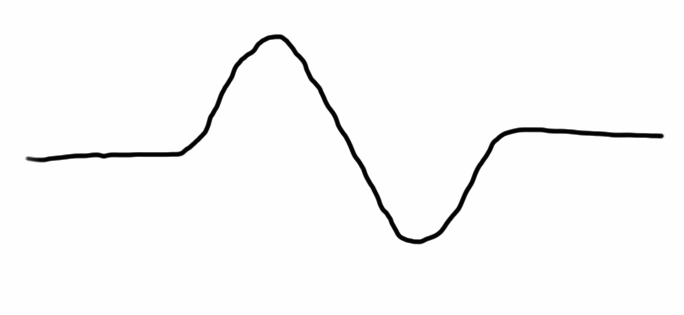
\includegraphics[width=0.7\columnwidth]{images/zigzag.png}
% \end{center}
% \caption{Zig-zag trajectory \TODO{This is hand-drawn, sorry about that... I will
% make a more professional-looking replacement}}
% \label{fig:zigzag}
% \end{figure}
 

% \subsection{Controller Composition}
% \TODO{Tarik and Jim write}
% \paragraph{Input}
% A configurations. A set of controllers. A control composition graph.
% \paragraph{Output}
% A composed controller if it is safe.
% \paragraph{Procedure}
% \begin{itemize}
% \item Compose the set of controllers based on the given control composition graph. Explain how the parallel composition and series composition are handled.
% \item\textbf{Check there is no controller conflict in the composition.}
% \item Execute the composed controller in user defined incremental time interval. At each time step, update each module position and check collision.
% \item \textbf{At each time step, check if the configuration will not have any unexpected behavior.}
% \end{itemize}

\subsection{ Verification of Configuration and Behavior}

\subsubsection{Verification of Configurations}\label{sec:verify_conf} In section~\ref{sec:conf_composition}, we introduced algorithms to compose a set of configurations into a single configuration. However, it might not be possible  or safe to form the structure represented by the composed configuration with the actual module. Consider the configuration shown in Figure~\ref{fig:smores_conf_collision}. It is easy to tell that such configuration is impossible to build with modules that allow only one connection at each node. Thus it is important to verify whether the configuration is valid or not for a given modular robot system.

\begin{figure}
\begin{center}
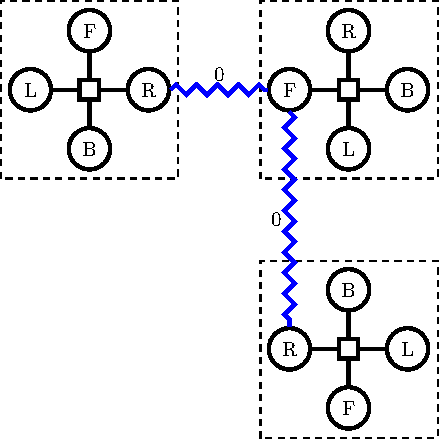
\includegraphics[width=0.5\columnwidth]{images/tikz/smores_conf_collision.pdf}
\end{center}
\caption{A configuration with self-collision \TODO{Should we call this self-collision?
 It's actually topologically flawed, which to me seems different than self-collision.}}
\label{fig:smores_conf_collision}
\end{figure}

\begin{definition}[Verification on Configuration]
Given a configuration $\mathcal{C}$ and state \(X_0\), we say $\mathcal{C}$ is valid in
state \(X_0\) if it satisfied the following set of properties:
\begin{itemize}
\item There is no collision between modules in the configuration.
\item The configuration is gravitationally stable.
\end{itemize}
Notice that in order to verify the validity of the configuration, one needs to know some properties of all modules for the given modular robot system, e.g. the geometry information, the mass of each module.
\end{definition}

\paragraph{Collision Checking} 
We obtain the positions and orientation of all modules through forward kinematics.
Using the known model geometry, we  check whether any two modules occupy the same space. If so, there exists a self-collision in the configuration.
\TODO{In general, this is a non-trivial problem to solve efficiently.  We should
briefly mention our method, and cite a reference to other available algorithms.}
\paragraph{Stability Checking}
 Gravitational stability is checked by computing the location of the center of mass of the configuration. For the given configuration $\mathcal{C}$
and state \(X_0\), the position of the center of mass is
\begin{equation*}
 P_{\mathcal{C}}=\dfrac{\sum\limits_{\mathcal{M}\in \gamma(\mathcal{C})}{P(\mathcal{M})\cdot \mathcal{M}_m}}{\sum\limits_{\mathcal{M}\in \gamma(\mathcal{C})}{\mathcal{M}_m}}
\end{equation*}
where $\mathcal{M}_m$ is the mass of the module $\mathcal{M}$, and \(P(\mathcal{M})\)
is a function returning the position coordinates of \(\mathcal{M}\) in the world frame.

We find the set of modules $M_c$ that have minimal position in the $z$ direction and consider them to
be the contact points between the ground plane and the configuration. We treat the
set \( \sigma = P(\mathcal{M})_i \forall \mathcal{M}_i \in M_c \ \) as an approximate set of contact points.
%A set of points in the $x$-$y$ plane can be extracted from $M_c$ as $\sigma=\{(\mathcal{M}.P.x, \mathcal{M}.P.y)\mid \mathcal{M} \in M_c\}$.
If projection of \(P_c\) onto the ground plane lies within the convex hull of \(\sigma\),
 configuration $\mathcal{C}$ is considered statically stable in state \(X_0\).

\subsubsection{Verification of Behavior}
In section~\ref{sec:behavior-representation}, we introduced a novel motion description language for modular robots. Actions defined by the language can be combined to produce more complex behaviors. Similar to configuration composition, we want to make sure the composed behaviors are valid and safe to execute. For example, a behavior that results in two modules colliding during the execution should be considered unsafe.

\begin{definition}[Verification on Behavior]
A behavior is valid if it satisfies the following set of properties when controlling a configuration of a given modular robot system
\begin{itemize}
\item There is no collision between modules at all time during the execution of the controller.
\item There is no behavior conflict at all time during the execution.
\item The configuration is gravitationally stable at the end of the execution.
\item The maximum duration when the configuration is not gravitationally stable during the execution is less than a time bound $t_{max}$.
\end{itemize}
\end{definition}
% State is the right term, so I deleted the TODO.
For a behavior with duration time $T_B$, we can check the state of the configuration with sampling time $t_B<t_{max}$. For each sample, we first detect behavior conflict by checking if different commands are given to the same joint of a module. If there is no behavior conflict, we can update the positions and orientations of all modules in the configuration based on behavior commands. Then we can check collision and gravitational stability of each configuration as we discussed in section~\ref{sec:verify_conf}. We argue that this behavior is not safe, if i) there are $n$ consecutive samples when the configuration is not gravitationally stable and $n\cdot t_B > t$; or ii) the configuration at time $T_B$ is not gravitationally stable.
%\subsection{Complexity}
%\TODO{Discuss the complexity of the algorithm with respect to the number of modules and size of gait tables.}

\section{Implementation }
\label{sec:example}
We implement a program to aid users to design and verify complex configurations and behaviors from a set of basic configurations and associated behaviors. We separated the program into two main parts, a configuration builder and a behavior builder.
Our implementation is built for the SMORES modular robot, but could easily be adapted
to other modular robot systems. \subsection{SMORES robot}
We have developed our system for the SMORES modular robot, developed at the
University of Pennsylvania \cite{Davey2012}. Each SMORES modules has four DoF
- three continuously rotating faces we call {\em turntables} and one
central hinge with a 180\textdegree\ range of motion (Figure~\ref{fig:SmoresRobot}). The
DoF marked 1, 2, and 4 have rotational axes that are parallel and coincident.
Each SMORES module can drive around as a two-wheel differential
drive robot.
SMORES modules may connect to one another via magnets on each of their four
faces, and are capable of  self-reconfiguration.
Formally, we denote the state of a SMORES module as \(X=\lbrace \theta_L, \theta_R,
\theta_F, \theta_B \rbrace\) and the set of attachment points as \(A=\lbrace L,R,T,B \rbrace\).




\begin{figure}[tb]
    \begin{center}
        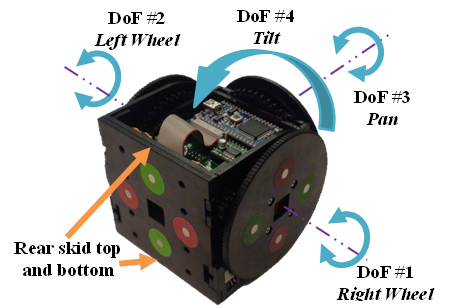
\includegraphics[width=\columnwidth]{images/smores_robot.png}
    \end{center}
    \caption{SMORES robot}
    \label{fig:SmoresRobot}
\end{figure}

\subsection{Configuration Builder}
Given a set of basic configurations, the configuration builder allows users to combine basic configurations by choosing connection node on each configuration, as demonstrated by green nodes in Figure~\ref{fig:gui_conf}. In addition, the configuration builder will warn users when the composed configuration is not valid without the usage of a physical simulator, e.g. Gazebo
\cite{koenig2004design}.

\subsection{Behavior Builder}
Given a composed configuration from the configuration builder, the behavior builder aids users in designing behaviors for the composed configuration by arranging a set of basic behaviors in parallel or in series. Figure~\ref{fig:gui_gait} illustrates a new behavior is composed by putting four basic behaviors in parallel. Similar to the configuration builder, the behavior builder will also warn users if there is self-collision in the configuration during the execution of composed behaviors without simulations in a physical engine.


\begin{figure}
\begin{center}
        \begin{subfigure}[b]{0.9\columnwidth}
                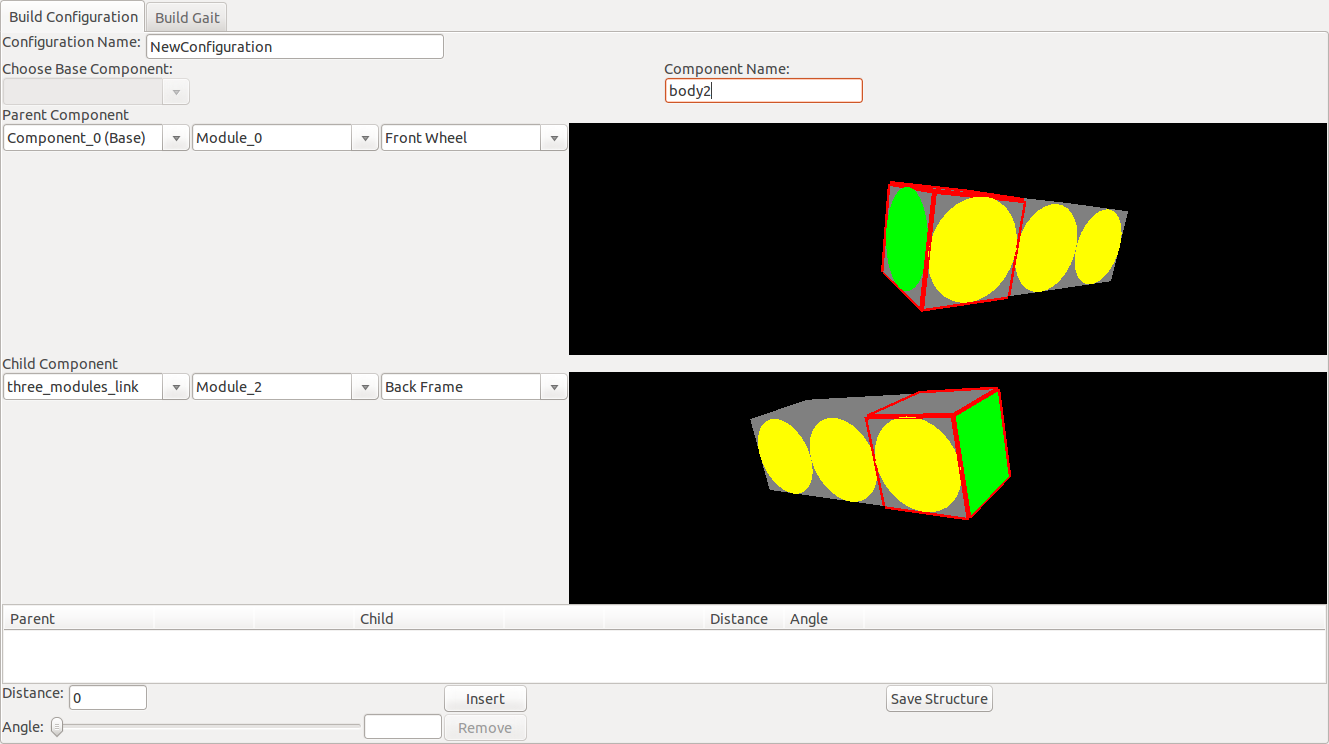
\includegraphics[width=\textwidth]{images/conf_window.png}
                \caption{GUI for configuration builder}
                \label{fig:gui_conf}
           \end{subfigure}
           
        \begin{subfigure}[b]{0.9\columnwidth}
                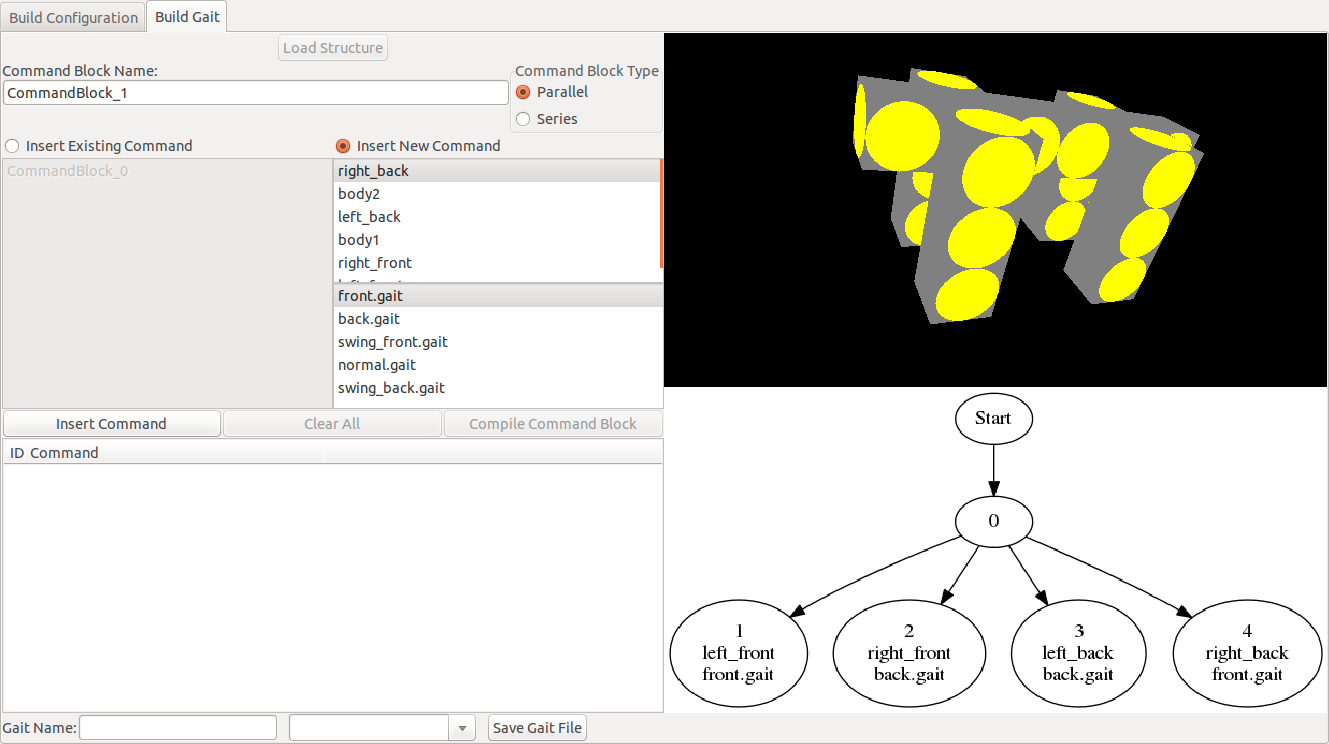
\includegraphics[width=\textwidth]{images/gait_window.png}
                \caption{GUI for behavior builder}
                \label{fig:gui_gait}
        \end{subfigure}
\end{center}
\caption{The program to design and verify configurations and behaviors}
\label{fig:smores_conf}
\end{figure}

% \TODO{Tarik and Jim write}\\
% With simulation in Gazebo:
% \begin{itemize}
% \item Show a configuration composed from a set of basic configurations.
% \item Show a composed controller that results in a collision in the configuration.
% \item Show an updated controller that resolves the collision
% \item Show a composed controller that results in an unexpected behavior.
% \item Show an updated controller that eliminates the unexpected behavior.
% \end{itemize}

\section{Examples}
Here we present some examples to illustrate important features of our framework.
\subsection{Toward a Standard Library}
Our eventual intention is to develop a large library of configurations and associated
behaviors which are available to all users of our framework, analogous to the standard
libraries of major programming languages.  The compositional nature of our framework
will allow users to rely heavily on the library when approaching new tasks, allowing
them to create sophisticated robots very quickly.

As a first step toward a standard library, we present a small library of configurations
and associated behaviors in Tables \ref{Order-1-configurations} and \ref{Order-2-configurations}.
Configurations in the library are organized by \textit{order}, defined recursively
as follows: a single module is an order-zero configuration, and the order of all
other configurations is one greater than the largest order of the sub-configurations
from which it is composed. Each configuration has an associated set of behaviors,
which the user can compose to accomplish tasks.  New behaviors for higher-order configuration can be created by composing the behaviors of its component sub-configurations.

For the library to be most effective, the set of configurations and behaviors available
 at each level (and especially at the lowest levels) should provide a rich set of
 functionalities without presenting the user with an overwhelming number of options. 
 Considering the small library in Tables \ref{Order-1-configurations} and \ref{Order-2-configurations},
 it is interested to note that a large  and diverse set of second- and third-order configurations can
be constructed from only one zero- and one first-order configuration. Developing metrics to
evaluate the quality of such a library is an interesting opportunity for future work. 

\begin{table*}
     \begin{center}
        \begin{tabular}{c c}
         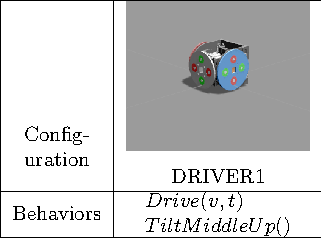
\includegraphics[scale=1]{images/library/tier0.pdf} &
         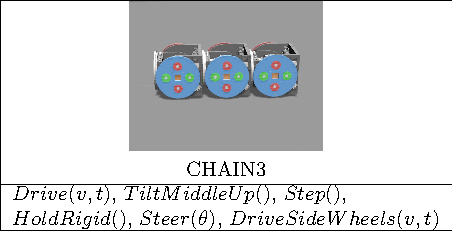
\includegraphics[scale=1]{images/library/tier1.pdf} \\
         \textbf{Order-0 (single module)} & \textbf{Order-1}
        \end{tabular}
         \caption{Order-0 and Order-1 configurations}
         \label{Order-1-configurations}
     \end{center}
\end{table*}
\begin{table*}
    \begin{center}
        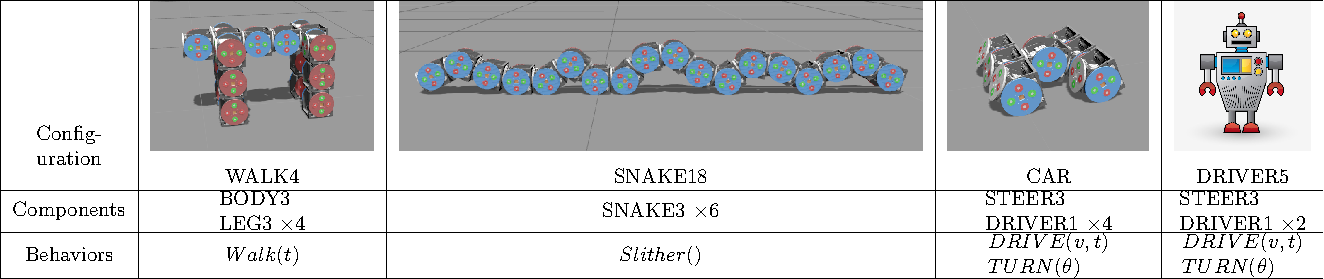
\includegraphics[width=\textwidth]{images/library/tier2.pdf}
        \caption{Order-2 configurations}
        \label{Order-2-configurations}
    \end{center}
\end{table*}
\begin{table*}
    \begin{center}
        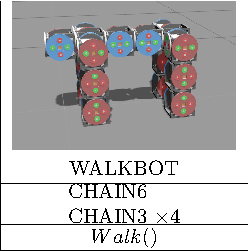
\includegraphics[scale=1]{images/library/tier3.pdf}
        \caption{Order-3 configurations}
        \label{Order-3-configurations}
    \end{center}
\end{table*}

\subsection{The User Perspective}
Figure~\ref{fig:design} demonstrates the design flow when a user is designing a configuration an its behaviors. We present the start-to-end user perspective in designing a complicated configuration called Walkbot. Consider a basic configuration formed by three modules in a line. We can form a ``body'' configuration by connecting two of the basic configurations as shown in Figure~\ref{fig:walkbot1}. With four more basic configurations and attach sides of those basic configurations to sides of the ``body'' configuration with certain angle offset, we can build a complex configuration, Walkbot, with four legs, as shown in Figure~\ref{fig:walkbot2}. Notice that by connecting multiple  basic configurations together, we can design a complex configuration without building with individual modules.

\begin{figure}
\begin{center}
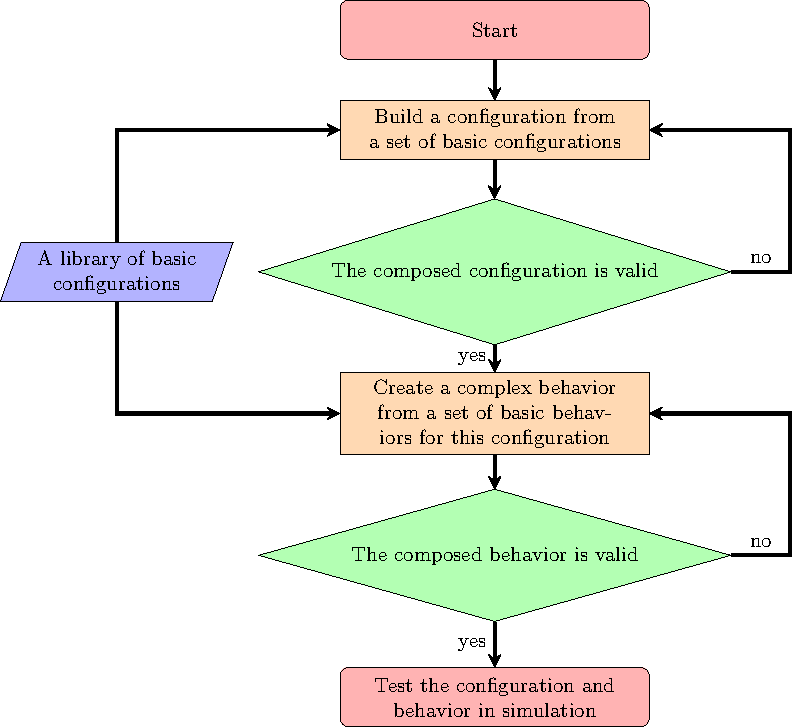
\includegraphics[width=0.9\columnwidth]{images/tikz/design_diagram.pdf}
\caption{The design flow}
\label{fig:design}
\end{center}
\end{figure}

\begin{figure}
\begin{center}
        \begin{subfigure}[b]{0.7\columnwidth}
                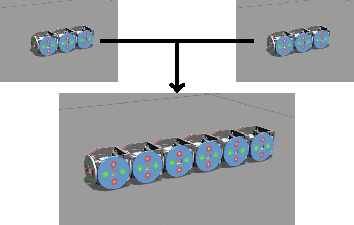
\includegraphics[width=\textwidth]{images/tikz/walkbot.pdf}
                \caption{Two identical configurations form a body}
                \label{fig:walkbot1}
           \end{subfigure}
           ~
        \begin{subfigure}[b]{0.9\columnwidth}
                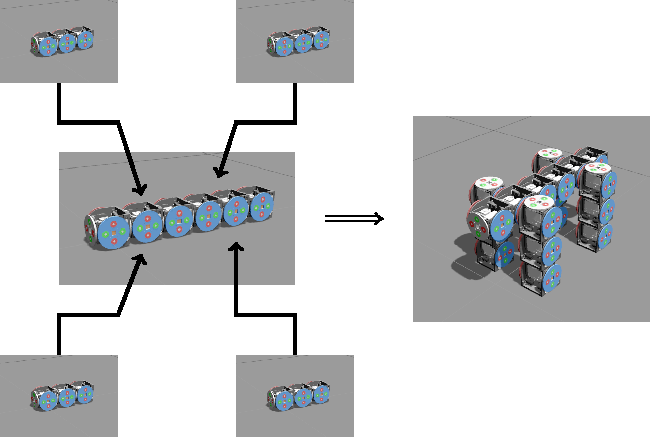
\includegraphics[width=\textwidth]{images/tikz/walkbot2.pdf}
                \caption{The body and four identical configurations form a Walkbot}
                \label{fig:walkbot2}
        \end{subfigure}
\end{center}
\caption{Building a Walkbot with six identical configurations}
\label{fig:walkbot}
\end{figure}

\subsection{Easy scale-up through composition}
Our framework allows users to quickly create and program large configurations. The
first-order CHAIN3 configuration (Figure \ref{fig:chain3}) can use a \(sineGait\)
behavior to locomote like a snake. Defining \(sineGait\)  as the series composition
of two half-waves will allow us to re-use the gait with larger snakes:
\begin{displaymath}
sineGait = Sc(~halfSine1,~halfSine2~)
\end{displaymath}
Arbitrarily long snake configurations can be created
by composing CHAIN3 configurations end-to-end; Figure \ref{fig:snake18} shows one with 18 modules.
A gait for an arbitrarily long snake is created by composing sine wave
gaits for each component in parallel, but with alternating phase:
\begin{align*}
nSnakeSineGait = ~~~~~~~~~~~~~~~~~~~~~~~~~~~~~~~~~~~~~~~~~~\\
Pc \left(~Sc\begin{pmatrix} halfSine1 \\ halfSine2 \end{pmatrix},
~Sc\begin{pmatrix} halfSine2 \\ halfSine1 \end{pmatrix},\ldots ~\right)
\end{align*}

\begin{figure}
        \begin{subfigure}{\columnwidth}
        \begin{center}
                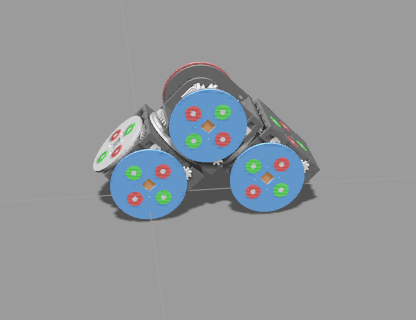
\includegraphics[width=1.5in]{images/library/snake3.png}
        \end{center}
                \caption{CHAIN3 (order 1)}
                \label{fig:chain3}
        \end{subfigure}
        \begin{subfigure}{\columnwidth}
                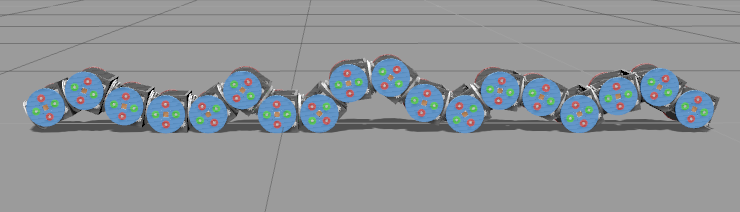
\includegraphics[width=\columnwidth]{images/library/snake18.png}
                \caption{SNAKE18 (order 2)}
                \label{fig:snake18}
        \end{subfigure}
\caption{CHAIN3 and SNAKE18 configurations}
\end{figure}

\subsection{Verification}
The need for verification becomes more important as design complexity increases.
 Consider the order-3 Backhoe design, composed of the order-2 car and PUMA arm configurations.
 It is easy for this design to become gravitationally unstable.  Our verification
 system warns the user when this happens. \TODO{We need to include pictures of this,
and flesh out this section.}

\section{Results}
In the past, designing configurations and behaviors to address new tasks has required
time on the order of one day \cite{sastra2011using}. Using our framework and library,
complex designs (such as the Walkbot or 18-module snake) can be created and programmed
in under an hour. \TODO{Mark, what is the best
way to present this comparison?} 

\section{Conclusions}
We worked hard, and had fun.

\section{Future}
\begin{itemize}
\item How to represent different attribute/ability of the configurations
\item Mention that we're going to run behaviors on actual hardware.
\end{itemize}




%% Use plainnat to work nicely with natbib. 

\bibliographystyle{plainnat}
\bibliography{references}

\end{document}















